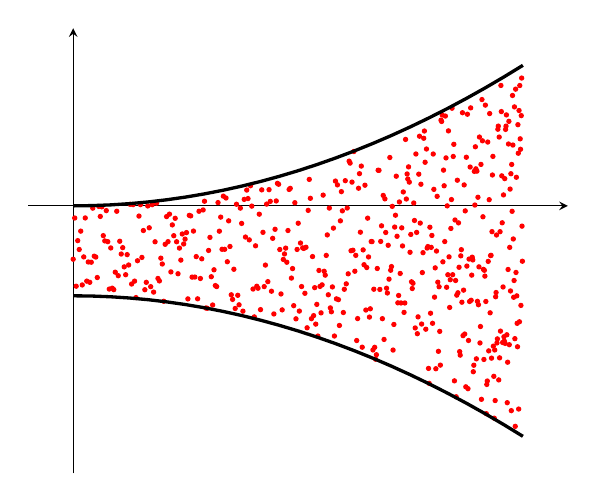
\begin{tikzpicture}[
    declare function={a(\x)=(\x/4)^2;},
    declare function={b(\x)=-(\x/4)^2-1;},
    declare function={f(\x) = 2*sqrt(2)*rad(atan(\x/(2*sqrt(2))))*5/2.99;}
]
	\begin{axis}[
	    domain=0:5, xmin=0,
	    axis lines=middle,
	    axis equal image,
	    xtick=\empty, ytick=\empty,
	    enlargelimits=true,
	    clip mode=individual, clip=false
	]
	\addplot [red, only marks, mark=*, mark size=0.75, samples=500]
	    (f(x), {0.5*(a(x)+b(x)) + rand * ( a(f(x)) - b(f(x))) / 2});
	\addplot [very thick] {a(x)};
	\addplot [very thick] {b(x)};
	\end{axis}
\end{tikzpicture}
